% Chapter Template

\chapter{Étude bibliographique} % Main chapter title

\label{ChapterX} % Change X to a consecutive number; for referencing this chapter elsewhere, use \ref{ChapterX}

%----------------------------------------------------------------------------------------
%	SECTION 1
%----------------------------------------------------------------------------------------

\section{Introduction}
Aujourd’hui, le domaine de l'image numérique est en pleine expansion. Depuis quelques années, avec l'explosion d'Internet et aussi le développement à grande échelle de la photographie numérique de haute qualité que nous observons ces dernières années dans de nombreuses activités quotidiennes, les bases de données d'images ont alors connues un développement énorme. Cette révolution numérique a cependant donné naissance à des nouvelles techniques de la structuration et du traitement d'image. Il s'agit donc de développer des méthodes mathématiques et des techniques capables de traiter une image numérique afin d’améliorer ou d’en extraire des informations jugées pertinentes, avec le but de baisser les coûts et rendre cette opération plus efficace.\\

Le contenu de ces images peut être décrit à deux niveaux différents:
 
\begin{itemize}
	\item Au niveau numérique, une image contient des pixels colorés dont on peut extraire des descripteurs de couleurs, des textures et des formes.
	
	\item Au niveau sémantique, une image peut être interprétée et peut avoir au moins un sens. 
\end{itemize}

Malheureusement, dans les systèmes d'information d'aujourd'hui, les images sont décrites numériquement alors que les utilisateurs s'intéressent à leur contenu sémantique, il est actuellement difficile de trouver des correspondances entre le niveau numérique et le niveau sémantique. Alors, l'utilisation et la gestion de ces bases d'images d'une manière efficace est très problématique, elle nécessite de nouvelles techniques de manipulation et de traitement des données. Dans ce contexte, la recherche d'images par le contenu s'intéresse à découvrir des connaissances implicitement contenues dans un ensemble de données en s'appuyant sur différentes approches qui peuvent être mises en œuvre indépendamment ou couplées. Ces techniques visent à explorer et à décrire le contenu des données, et à en extraire l'information la plus importante et la plus significativement pertinente.
%
%Bien que plusieurs années de travaux scientifiques en recherche d’images par le contenu, ont d’ores et déjà permis la réalisation et le développement des systèmes performants, permettant plusieurs formes et techniques d’indexation par analyse du contenu, mais ce domaine demeure encore aujourd’hui un sujet très ouvert et actif dans la communauté internationale depuis plus d’une dizaine d'années.
\\

Ce chapitre s’inscrit dans ce cadre qui porte un aperçu sur les images numériques et ces caractéristiques. Ensuite, nous allons donner des notions de base du domaine de traitement d'image numérique. Puis nous présenterons le principe général des systèmes CBIR.


%-----------------------------------
%	SECTION 1
%-----------------------------------

\section{Représentation machine du contenu visuel des images}

Avant d'entrer dans le vif du sujet, il est important de comprendre la nature des objets que nous allons manipuler. Intéressons-nous à la notion d'image, qu'est-ce qu'une image?

Une des plus anciennes définitions de l'image est celle donnée par Platon [Platon] : « J'appelle image d'abord les ombres ensuite les reflets qu'on voit dans les eaux, ou à la surface des corps opaques, polis et brillants et toutes les représentations de ce genre ». En informatique, une image est une représentation numérique en mémoire d’un sujet imprimé sur une rétine artificielle (matricielle comme le capteur d’un appareil photographique numérique ou la scène virtuelle d’une image de synthèse ou bien linéaire comme le capteur optique du télécopieur, du photocopieur ou du scanner). \\

On distingue deux types d'images à la composition et au comportement différent: images matricielles et les images vectorielles.

\subsection{Images matricielles (bitmap)}
Les images matricielles sont des images numériques qui stockent les informations sous la forme d'une matrice, des points à plusieurs dimensions, chaque dimension représentant une dimension spatiale (hauteur, largeur), ou autre (niveau de résolution). Dans le cas des images à deux dimensions, les points sont appelés pixels. 

\begin{figure}[H]
	\centering
	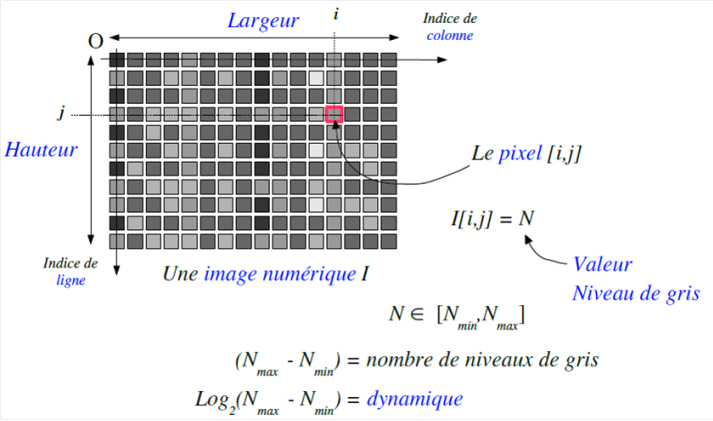
\includegraphics[width=0.7\textwidth]{Figures/pixel} 
	\caption{Image numérique au niveaux de gris: notion de pixel.}
\end{figure}


Un pixel $(i, j)$, ( i est l'indice de la ligne et j est l'indice de la colonne), possède une valeur $I(i, j)$ qui peut être un scalaire représentant la valeur du niveau de gris du pixel (dans le cas des images noir et blanc ou des images en niveaux de gris), ou un vecteur représentant les trois canaux de la couleur du pixel (dans le cas des images couleurs).\\

Ces images peuvent être regroupées en plusieurs catégories:



%-----------------------------------
%	SUBSECTION 1
%-----------------------------------

\subsubsection{Image à niveaux de gris}
 Les images à niveaux de gris sont composées de pixels de valeurs scalaires représentant la luminosité/intensité. En général ces valeurs des pixels sont  codés sur $n$ bits, ce qui lui confère des valeurs entières comprises entre 0 et $2^n-1$, 0 et 255 si $n = 8$. Dans ce cas, le pixel est codé sur un octet (nous disposerons ainsi de $2^8=256$ couleurs). La valeur 255 correspond au blanc, et la valeur 0 correspond au noir. Les valeurs intermédiaires correspondent à des niveaux de gris allant du noir au blanc.\\

La figure 1.1 ci-dessous montre une sous-matrice de $5 \times 5$ pixels extrait d’une image. Nous pouvons voir les valeurs qui composent la sous-matrice et les niveaux de gris qui permettent d’afficher l'image.

\begin{figure}[H]
	\centering
	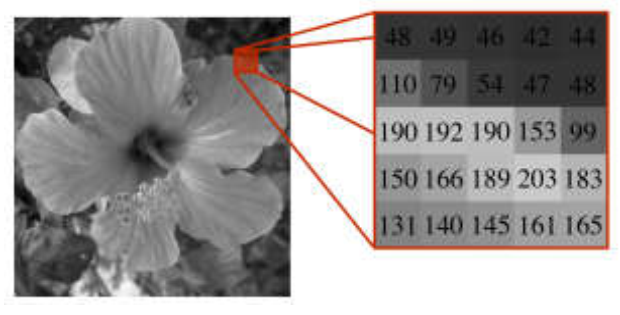
\includegraphics[width=0.4\textwidth]{Figures/gray} 
	\caption{Image à niveaux de gris.}
\end{figure}

\begin{figure}[H]
	\label{fig:tableRVB}
	\centering
	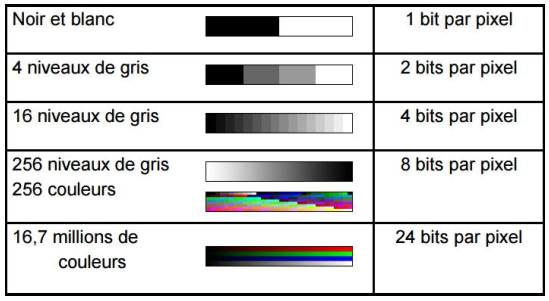
\includegraphics[width=0.65\textwidth]{Figures/tableRVB} % Include the image .png
	
	\caption{Représentation des pixels en fonction de nombre des bits.}
	
\end{figure}
%-----------------------------------
%	SUBSECTION 2
%-----------------------------------
\subsubsection{Image couleur}
Une image couleur est composée de pixels dont les valeurs sont en général multicomposantes. En effet, nous pouvons citer parmi les formats les plus utilisés pour représenter la valeur du pixel, le triplet (R,V, B) ou (R,G,B) où R, G et B sont respectivement les valeurs des composantes rouge, verte et bleu du pixel. Chaque composante du triplet est représentée par un entier variant entre 0
(absence de la composante) et 255 (intensité maximale). 

\begin{figure}[H]
	\centering
	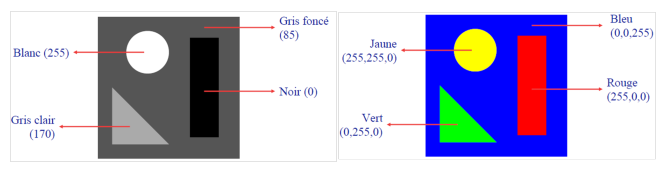
\includegraphics[width=0.6\textwidth]{Figures/grayvscol} 
	\caption{Image à niveaux de gris VS Image couleur.}
\end{figure}

Le triplet (0, 0, 0) correspond au noir, (255, 0, 0) au rouge, (255, 255, 0) au jaune et (255, 255, 255) au blanc.  Dans ce cas, le pixel est codé sur trois octets. Une image couleur RVB ou (RGB) possède trois composantes tandis qu'une image en niveaux de gris n’en possède qu’une seule. En d'autre termes, Une image couleur correspond à la synthèse additive de 3 images, rouge, vert et bleu. Chaque pixel est donc codé sur $3 \times n = 24 $ bits.

\begin{figure}[H]
	\centering
	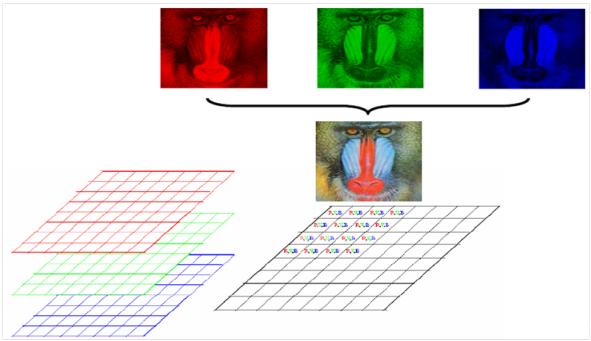
\includegraphics[width=0.6\textwidth]{Figures/rgb} 
	\caption{Image couleur dans l’espace RGB.}
\end{figure}

\subsection{Images vectorielles}
Les images vectorielles, contrairement aux images matricielles, contiennent les primitives de dessin (formes, position, couleurs...) des objets géométriques qu’elles représentent (segments de droite, polygones, arcs de cercles...). Ces images sont essentiellement utilisées pour réaliser des schémas ou des plans. Leur codage dépend directement du logiciel qui a permis de les créer. Ces images présentent deux avantages: elles occupent peu de place en mémoire et peuvent être facilement redimensionnées sans perte d'information (peuvent être agrandies à volonté sans perte de qualité).

\begin{figure}[H]
	\centering
	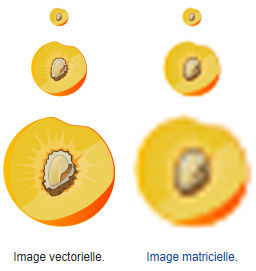
\includegraphics[width=0.3\textwidth]{Figures/vecteur} 
	\caption{Une image vectorielle: redimensionnable sans perte de qualité, contrairement à une image matricielle.}
\end{figure}



%-----------------------------------
%	SECTION 2
%-----------------------------------
\section{Formats d'images numériques}
Un format d'image est une représentation informatique, associée à des informations sur la façon dont l'image est codée et fournissant éventuellement des indications sur la manière de la décoder et de la manipuler. La plupart des formats sont composés d'un en-tête contenant des attributs (dimensions de l'image, type de codage, etc.), suivi des données de l'image. La structuration des attributs et des données diffère pour chaque format d'image [MM11].

\begin{table}[H]
	\centering
	\caption{Les différents formats des images matricielles.}
	\begin{tabular}{|l|l|l|l|}
		
		\hline
		\textbf{Format} & \textbf{Avantages} &
		\textbf{Inconvénients} & \textbf{Caractéristiques} \\
		\hline
		\makecell{JPEG : Joint\\
			Photographic\\
			Experts Group\\
			(extension
			.jpg)}
		& \makecell{Excellente\\
			compression\\
			avec la\\
			possibilité de\\
			sélectionner le\\
			taux} 
		& \makecell{Compression\\
			détruit la qualité.}
		&  \makecell{Le format le plus\\
			courant.\\
			Il ne supporte pas\\
			un fond transparent.\\
			Spécialement conçu\\
			pour les\\
			photographies.}   \\
		\hline
		
		\hline
		\makecell{GIF :
			Graphics\\
			Interchange\\
			Format\\
			(extension .gif)}
		& \makecell{Supporte\\
			l'animation et la\\
			transparence.\\
			Taux de\\
			compression\\
			élevé.} 
		& \makecell{Les couleurs\\
			sont définies sur\\
			une palette de\\
			256 couleurs.}
		&  \makecell{Utilisé généralement\\
			pour des photos de\\
			type dessin. Occupe\\
			peu d'espace disque.\\
			Presque tous les\\
			navigateurs peuvent\\
			le soutenir.}   \\
		\hline
		
		\hline
		\makecell{PNG : Portable\\
			Network\\
			Graphics\\
			(extension
			.png)}
		& \makecell{Emploie la\\
			compression\\
			sans perte de\\
			données,\\
			possibilité de\\
			transparence.} 
		& \makecell{Un peu plus\\
			lourd qu’un jpg\\
			donc il n’est pas\\
			très efficace pour\\
			les larges\\
			photographies.}
		&  \makecell{Format destiné à\\
			améliorer la\\
			limitation du\\
			format GIF. Appelé à\\
			devenir le futur\\
			standard internet.}   \\
		\hline
		
%	
%		\makecell{TIFF : Tagged\\
%			Image File\\
%			Format\\
%			(extension .tif)}
%		& \makecell{Il permet\\
%			d'obtenir une\\
%			image de très\\
%			bonne qualité,\\
%			possible\\
%			d’ajouter une\\
%			couche de\\
%			transparence.} 
%		& \makecell{Taille\\
%			volumineuse. Un\\
%			choix à éviter\\
%			pour le Web\\
%			puisqu'aucun\\
%			navigateur Web\\
%			ne le lit\\
%			directement.}
%		&  \makecell{le format le plus\\
%			couramment utilisé\\
%			pour stocker des\\
%			images.\\
%			Dédié pour les\\
%			professionnels\\
%			et pour l’impression\\
%			commerciale.}   \\
%		\hline
%		
%		\makecell{BMP : BitMaP\\
%			(extension
%			.bmp)}
%		& \makecell{Format natif de\\
%			windows. Pas de\\
%			perte de qualité.} 
%		& \makecell{Utilisable\\
%			uniquement sur\\
%			la plateforme\\ de
%			Microsoft. Taille\\
%			volumineuse.}
%		&  \makecell{Peu utilisé sur\\
%			le web.\\
%			Gère les palettes\\
%			pour les couleurs en\\
%			mode indexées.}   \\
%		\hline
	\end{tabular}
\end{table}


\begin{table}[H]
	\centering
	\caption{Les différents formats des images vectorielles.}
	\begin{tabular}{|l|l|l|l|}
		
		\hline
		\textbf{Format} & \textbf{Avantages} &
		\textbf{Inconvénients} & \textbf{Caractéristiques} \\
		\hline
		\makecell{AI : Adobe\\
			Illustrator \\(extension .ai)}
		 & \makecell{Reconnu par\\
			tous\\
			les logiciels\\
			graphiques.} & \makecell{Format propres\\ a
		Adobe Illustrator.}
		&  \makecell{Format développé\\
			par Adobe Systems.\\
			L'un des plus\\
			repandu pour la\\
			création de logotypes.}   \\
		\hline
		
		\makecell{EPS :
			Encapsulated\\
			Postscript\\
			(extension
			.eps)}
		& \makecell{Peut être\\
			visualisé et\\
			importé dans\\
			bon nombre de\\
			logiciels de\\
			dessins.} 
		& \makecell{Destinés qu'à\\
			l'impression.\\
			Fichier très\\
			lourd.}
		&  \makecell{EPS est un fichier PS\\
			qui comporte\\
			quelques restrictions\\
			supplémentaires. Le\\
			plus utilisé pour\\
			transférer une image\\
			ou une illustration.}   \\
		\hline
	
		\makecell{SVG : Scalable\\
			Vector\\
			Graphics\\
			(extension\\
			.svg)}
		& \makecell{Extensible car il\\
			est basé sur\\
			XML. Permet les\\
			animations et la\\
			transparence.} 
		& \makecell{Manque\\
			d'implémentation\\
			au sein de\\
			navigateurs\\
			(besoin d'un\\
			plugin).\\
			Production de\\
			code\\
			volumineux.}
		&  \makecell{Il est utilisé sur les\\
			mobiles, et souvent\\
			pour la création de\\
			"schémas,\\
			diagrammes ou\\
			cartes".}   \\
		\hline
%		
%		\hline
%		\makecell{SWF : Small\\
%			Web Format\\
%			(extension\\
%			.swf)}
%		& \makecell{Il est idéal pour\\
%			la publication\\
%			sur le web. Peut\\
%			contenir des\\
%			animations, mp3\\
%			et des JPEG.} 
%		& \makecell{Format\\
%			propriétaire.}
%		&  \makecell{Format spécifique à\\
%			Flash et accepté par\\
%			la majorité\\
%			des configurations\\
%			actuelles. Contrôler\\
%			par Adobe.}   \\
%		\hline
%		
%		\hline
%		\makecell{PICT : Picture\\
%			(extension\\
%			.pict)}
%		& \makecell{Créé par Apple\\
%			comme standard\\
%			pour ses\\
%			premiers\\
%			Macintosh.} 
%		& \makecell{Disponible\\
%			uniquement sur\\
%			les équipements\\
%			d'Apple.}
%		&  \makecell{Remplacé par d'autre\\
%			format en tant que\\
%			métaformat natif.}   \\
%		\hline
	\end{tabular}
	
\end{table}

%-----------------------------------
%	SECTION 3
%-----------------------------------
\section{Les caractéristiques d’une image numérique}
Les images numériques sont également définies par des propriétés appelées les caractéristiques globales, permettant généralement de mieux rendre compte de certaines propriétés visuelles de l'image, elles sont utilisées pour des traitements ultérieurs entrant dans le cadre d'applications telles que la détection d'objets ou la recherche d'images par le contenu par exemple.
Les caractéristiques globales d’une image numérique :

\subsection{Le Pixel}
Le pixel provient d’une abréviation de l’expression anglaise PICture Element (souvent abrégé px). C’est l'unité de base permettant de mesurer la
définition d'une image numérique matricielle.
L'ensemble de ces pixels est contenu dans un tableau à deux dimensions
constituant l'image finalement obtenue avec une couleur associée à chaque
pixel. Un pixel est si petit qu'on le voit à peine à l'œil nu, cela permet d'en
afficher beaucoup et d'avoir une image nette.

\subsection{La dimension}
La dimension ou la définition d’une image numérique, est le nombre total de pixels composant cette image. Il suffit de calculer le produit : largeur [px] * hauteur [px] pour déterminer la dimension. Par exemple : une image
avec une largeur = une hauteur = 8 pixels, La dimension = 8 * 8 = 64 pixels.

\begin{figure}[H]
	\centering
	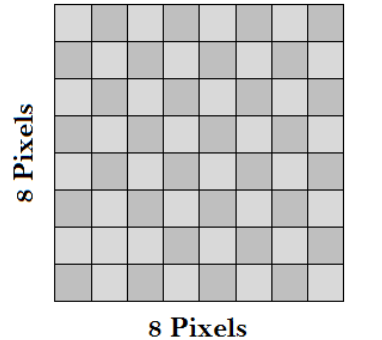
\includegraphics[width=0.3\textwidth]{Figures/dim} 
	\caption{La dimension d’une image.}
\end{figure}

\subsection{La résolution}
La résolution est la densité de l’image en pixels une fois reproduite,
mesurée en « ppi » (pixels per inch) ou en français « ppp » (pixels par pouce).
Elle décrit la clarté ou la finesse des détails d’une image matricielle. Plus le nombre de pixels par pouce est grand, plus la résolution est élevée.
Généralement, une image haute résolution produit une impression de
meilleure qualité.

\subsection{La couleur}
La couleur est la perception visuelle que nous avons des différentes
longueurs d’onde qui constituent la lumière visible. Cette partie du spectre
de la lumière s'étend du violet (4000 angströms) au rouge (7000 angströms),
les autres ne sont pas perçues.
Dans les systèmes de recherche d’image par le contenu, la couleur est
l'information visuelle la plus utilisée en raison de son invariance par rapport à l'échelle. 

Une couleur est généralement représentée par trois composantes. Ces composantes définissent un espace de couleurs. Il existe plusieurs espaces colorimétriques qui ont chacun certaines caractéristiques
intéressantes, le plus couramment utilisé est le système RGB.
\subsubsection{Espace des couleurs}
Une couleur est généralement représentée par trois composantes. Ces composantes définissent un espace des couleurs. On peut citer l'espace RVB, l'espace CIE (Commission Internationale de l'Eclairage) XYZ ou Yxy, ou encore l'espace Lab. Selon l'espace de couleurs choisi pour représenter une image couleur, le nuage des couleurs (c'est à dire l'ensemble des couleurs de l'image) n'aura pas la même répartition dans l'espace 3D.


\begin{figure}[H]
	\label{fig:espaceRVB}
	\centering
	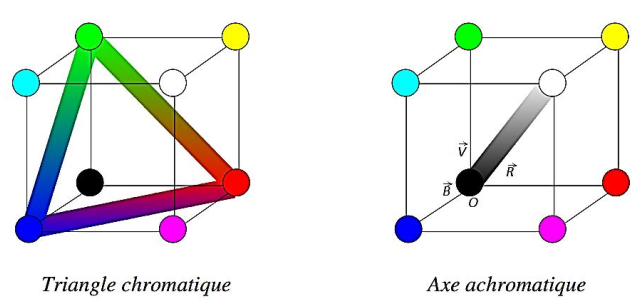
\includegraphics[width=0.65\textwidth]{Figures/espaceRVB} % Include the image .png
	\caption{Espace de couleur RVB.}
\end{figure}

Les espaces de couleurs classiques, tels que le RVB, CIE XYZ, ...etc, sont issus d'une approche purement physique, sans la prise en compte de données psychophysiques. Dans d'autre espaces de couleur, tels que l'espace Lab, l'approche physique est corrigée selon des données de la vision humaine.\\

De nombreuses méthodes de descriptions d'images proposent de caractériser la couleur dans certains espaces couleurs pour profiter des propriétés de ces derniers. La figure 1.9 montre les principaux espaces couleurs utilisés en indexation d’images [Ouhda19].
\begin{figure}[H]
	\label{fig:espaceCouleur}
	\centering
	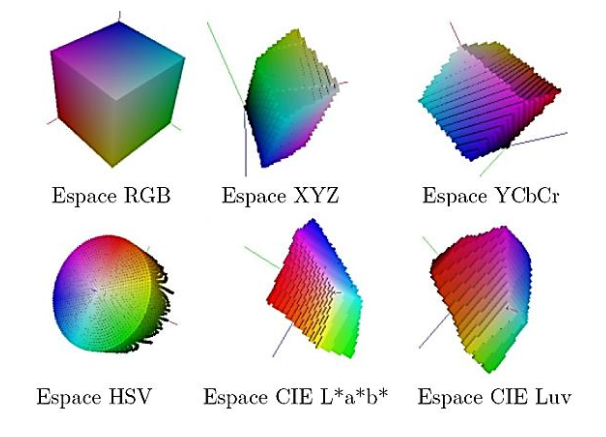
\includegraphics[width=0.45\textwidth]{Figures/espaceCouleur} % Include the image .png
	\caption{Les principaux espaces couleurs utilisés en indexation d'images.}
	
\end{figure}

On peut principalement citer :
\begin{itemize}
	\item \textbf{RGB} (Rouge, Vert, Bleu): est le plus utilisé car la plupart des images originelles sont codées dans cet espace couleur, ce qui ne nécessite pas de transformation inter espace couleur, donc facilement applicable.
	
	\item \textbf{HSV}: chaque composante représente respectivement la teinte, la saturation et la luminance.
	
	\item \textbf{YCbCr}: est utilisé dans les normes MPEG 1, 2 et 4, ses composantes sont décorrélées et de faibles dynamiques, ce qui permet de bons taux de compression.
	
	\item \textbf{L*a*b*} ou \textbf{CIE Luv}: sont des espaces couleurs perceptuellement uniformes. Ces espaces ont été créés dans le but de rendre plus homogène l’espace des couleurs et de
	permettre de mesurer uniformément les distances entre couleurs en tout point de l'espace. Deux couleurs proches dans ces espaces couleurs sont proches perceptuellement. Ces espaces sont grandement utilisés dans les systèmes de comparaison d'images.
\end{itemize}

\subsection{Contours et Textures}
Les contours représentent la frontière entre les objets de l’image, ou la
limite entre deux pixels dont les niveaux de gris représentent une différence significative [ZZ18]. Une texture se caractérise par la répétition d’un motif ou de quelques éléments. Plus précisément, la texture peut être vue comme un ensemble de pixels (niveaux de gris) spatialement agencés selon un certain nombre de relations spatiales, ainsi créant une région homogène [ZZ18]. On peut ainsi grâce à la texture faire la différence entre un coucher du soleil et une orange. Elle traduit donc l’aspect homogène d’une zone et peut être décrite selon ses propriétés spatiales et fréquentielles.\\

Dans le deuxième chapitre nous allons étudier la textures avec plus de détails.

\subsection{Luminance et Contraste}

\begin{itemize}
	\item \textbf{Luminance :}
	C’est le degré de luminosité des points de l’image. Elle est définie aussi comme étant le quotient de l’intensité lumineuse d’une surface par l’aire apparente de cette surface. Pour un observateur lointain, le mot luminance est substitué au mot brillance, qui correspond à l’éclat d’un objet.
	Dans le système international d'unités, la luminance s'exprime en candela par mètre carré, symbole ($cd/m^2$) [ZZ18].
	
	\item \textbf{Contraste :}
	C’est l’opposition marquée entre deux régions d’une image, plus
	précisément entre les régions sombres et les régions claires de cette image.
	Le contraste est défini en fonction des luminances de deux zones d’images (elle différencie les couleurs claires des couleurs foncées).
	Si $ L_1 $ et $ L_2 $ sont les degrés de luminosité respectivement de deux zones voisines $ A_1 $ et $ A_2 $ d’une image, le contraste $ C $ est défini par le rapport [ZZ18]:
	\begin{equation}
		 C = \frac{L_1 - L_2}{L_1 + L_2} 
	\end{equation}
\end{itemize}
 

 

\subsection{Le bruit}
Un bruit dans une image est considéré comme un phénomène de brusque
variation de l’intensité d’un pixel par rapport à ses voisins, il provient de l’éclairage des dispositifs optiques et électroniques du capteur.
Le bruit peut provenir de différentes causes :
\begin{itemize}
	\item Environnement lors de l'acquisition,
	\item Qualité du capteur,
	\item Qualité de l'échantillonnage.
	\item Ajouter par des techniques de traitement d'image numérique.
\end{itemize}


 
%-----------------------------------
%	SECTION 4
%-----------------------------------
\section{Traitement d'image numérique}
Le traitement d'image est l’ensemble d’opérations qui permettent
l’amélioration (filtrage, ...), la modification (rotation, symétrie) et l’extraction de l’information à partir des images numériques.
D'autre étapes sont nécessaires avant de commencer le traitement d’image
tel que :
\begin{itemize}
	\item L’acquisition et la numérisation de l’image par des dispositifs comme les scanners, les appareils photo qui permettent d’effectuer l’échantillonnage et la quantification d’une image.
	
	\item Il est facile d’effectuer les différentes opérations de traitement d’images grâce à des outils informatiques qui sont installés sur une unité centrale.
	
	\item Le stockage de l’image numérisée sur un support informatique (disque dur, CD-ROM, Clé USB, etc).
	
	\item L’affichage grâce à des dispositifs de visualisation qui permet l’affichage des images traités.
\end{itemize}

\begin{figure}[H]
	\centering
	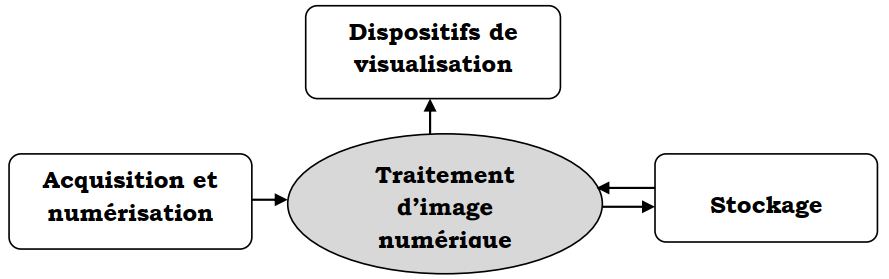
\includegraphics[width=0.6\textwidth]{Figures/tin} 
	\caption{Architecture d'un système de traitement d’image.}
\end{figure}

\subsection{Filtrage}
Les images numériques telles qu'elles sont acquises, sont très souvent
inexploitables pour le traitement d'images. Elles contiennent des signaux
bruités. Il est donc souvent nécessaire d'améliorer sa qualité. Deux types
d’améliorations des images sont possibles :

\begin{itemize}
	\item \textbf{Amélioration du rapport signal sur bruit :} La méthode la plus simple pour augmenter le rapport signal/bruit consiste à appliquer le principe des analyseurs multicanaux, c'est-à-dire effectuer plusieurs acquisitions de l’image (n par exemple) : ce qui revient à effectuer plusieurs sommations du signal. Le bruit n’apparaissant statistiquement jamais au même endroit, sera uniformément réparti, alors que le signal, apparaissant toujours au même endroit, sera amplifié d’un facteur racine carrée de n [ZZ18].
	
	Généralement, l'amélioration du rapport signal/bruit n’est pas suffisante pour obtenir une très bonne qualité, ce qui nécessite d’ajouter une deuxième amélioration que l’on appelle une opération de filtrage (ou lissage).
	
	\item \textbf{Amélioration par filtrage :}
	L'objectif avoué du filtrage est de réduire les variations d'intensité au sein de chaque région de l'image tout en respectant l'intégrité des scènes :
	les transitions entre régions homogènes, les éléments significatifs de l'image	doivent être préservés au mieux. Différentes méthodes de filtrage ont été développées suivant le type et l’intensité du bruit, ou les applications auxquelles on destine l'image.\\
	
\end{itemize}

Deux approches sont possibles dans la conception d’un filtre d’image.
La première consiste à construire un opérateur qui fonctionne de manière
linéaire et invariante dans le décalage. Ces filtres, au sens propre du terme, sont appelés filtres linéaires. L'alternative consiste à ne plus imposer au filtre de procéder de façon linéaire ou de façon invariante dans le décalage. On peut construire dans cette hypothèse un très grand nombre d’opérateurs que nous regroupons sous le terme de filtres non linéaires.

\subsubsection{Filtres linéaires}
Un filtre linéaire transforme un ensemble de données d'entrée en un
ensemble de données de sortie selon une opération mathématique appelée
convolution. Lorsqu'il s'agit de données numérisées comme dans le cas du
traitement d'image, la relation entre les valeurs des pixels de sortie et celle des pixels d'entrée est décrite par un tableau de nombres, généralement carré, appelé matrice de convolution. Le filtre local est dit linéaire si la valeur du nouveau pixel est une combinaison linéaire des valeurs des pixels du voisinage.

Un exemple des filtres linéaires est :
\paragraph{ $\bullet$ Filtre gaussien :}
L’expression gaussienne en deux dimensions est donnée par :
\begin{equation}
  G(x, y) = \frac{1}{2\pi \sigma^2} \exp(-\frac{(x-\mu)^2+(y-\mu)^2}{2 \sigma^2})
\end{equation}
Où x et y représentent les distances sur les deux axes, $\sigma$ et $\mu $ sont respectivement la moyenne et l’écart-type de la distribution gaussienne. L’intérêt de ce filtre est que l’on contrôle facilement le degré de filtrage à travers le paramètre $\sigma$. En numérique, le filtre est représenté mathématiquement par une matrice. La convolution qui permet de traiter l'image s'effectue de manière très simple.

Le pixel à traiter étant placé sur le centre du filtre, on multiplie les
coefficients du filtre par les valeurs des pixels correspondants et on calcule la moyenne qui est éventuellement pondérée. La discrétisation de ce filtre de la moyenne $\mu = 0$  et d’écart-type $\sigma = 0.6$. donne le masque suivant :

\begin{figure}[H]
	\centering
	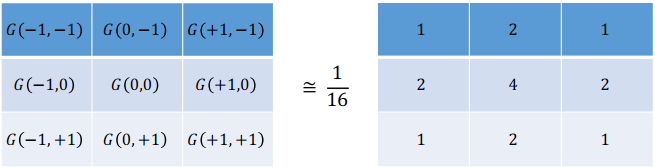
\includegraphics[width=0.5\textwidth]{Figures/gaussien} 
	\caption{Approximations discrètes de la distribution gaussienne de
		moyenne $\mu = 0$  et d’écart-type $\sigma = 0.6$.}
\end{figure}

\subsubsection{Filtres non linéaires}
Ils ont été développés pour régler l’insuffisance des filtres linéaires
surtout la mauvaise conservation des contours mais ils ont le défaut
d’imposer des déformations irréversibles à l’image. Leur principe est le même
que celui des filtres linéaires, il s’agit toujours d’utiliser des opérateurs
recherchant des valeurs de pixels extrémales au sein d’un voisinage.
Un exemple des filtres non linéaires est :

\paragraph{ $\bullet$ Filtre médian:}
Il appartient à la famille des filtres d’ordre. Le principe de ce filtre est de remplacer chaque valeur de pixel central par la valeur de pixel médiane observée dans leur voisinage. Cette valeur médiane permet d’éviter de procéder à des moyennes de valeurs de pixels de natures différentes. Son objectif est de réduire le bruit impulsionnel et préserver les contours.
\begin{figure}[H]
	\centering
	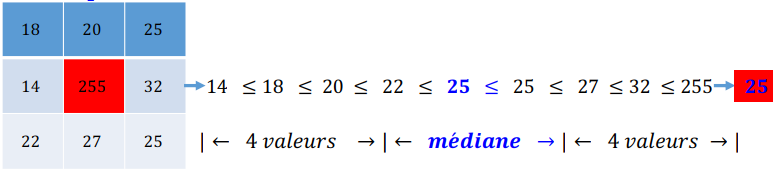
\includegraphics[width=0.6\textwidth]{Figures/median} 
	\caption{Principe du filtre médian.}
\end{figure}

\subsection{Détection de contour}
La détection de contour est une étape préliminaire à de nombreuses
applications de l'analyse d'images dans le but de repérer les points d’une
image numérique qui correspondent à un changement brutal de l’intensité
lumineuse. La détection des contours réduit de manière importante la
quantité de données et élimine les informations qu'on peut juger moins
pertinentes, tout en gardant les attributs importants de l'image.
Un contour se matérialise par une rupture d'intensité dans l'image
suivant une direction donnée. Ces changements d’intensités permettent de
décrire des variations importantes qui se traduisent par des discontinuités
dans la profondeur, dans l'orientation d'une surface, dans les propriétés
d'un matériau et dans l'éclairage d'une scène.\\

Il existe de nombreux filtres pour trouver les contours des objets. Ces filtres transforment l'image d'entrée en une image noire sauf aux points où un contour est détecté qui est marqué en blanc. Voici quelques exemples des filtres utilisés pour la détection de contour.

\begin{itemize}
	\item \textbf{Filtre de Prewitt :}
	Le filtre de Prewitt introduit un flou, chacune des deux matrices étant le produit du filtre dérivation dans la direction considérée par un filtre de flou	rectangulaire selon l'autre direction.
	
	\item \textbf{Filtre de Sobel :}
	La technique précédente est améliorée en remplaçant le filtre rectangulaire par un filtre triangulaire.
	
	\item \textbf{Filtre de Canny :}
	C’est un filtre de Sobel précédé par un lissage gaussien et suivi par un seuillage. 
	
\end{itemize}
\begin{figure}[H]
	\centering
	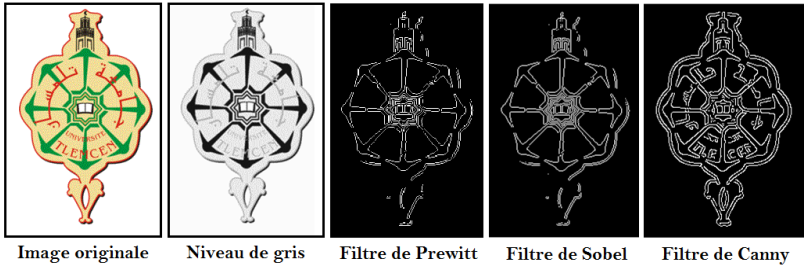
\includegraphics[width=0.5\textwidth]{Figures/conrour} 
	\caption{Détection de contour par les différents filtres.}
\end{figure}

\subsection{Segmentation}
La segmentation est une étape importante dans le traitement d'image numérique.
Elle consiste de partitionner l’ensemble des pixels de l'image entre eux selon des critères prédéfinis en différents régions connexes, qui constituent un pavage ou une partition de l'image, chaque région est supposée correspondre à un objet.
Lorsqu’un homme regarde une image, il peut séparer et reconnaitre les
objets situés dans cette image grâce à ces connaissances de haut niveau
(compréhension des objets et de la scène). Par exemple, si on travaille sur
une image d’un bureau, nous allons reconnaître facilement les ordinateurs,
les tables et les chaises. Contrairement, les machines informatiques ont
besoin des algorithmes bien développés pour faire la segmentation.
En effet, de nombreuses techniques ont été trouvées selon le type d’image
sur laquelle on travaille, et selon la nature des outils de segmentation
utilisés, certain sont plus performantes que d’autres, mais comme nous
allons le voir, les plus souvent sont destinées à un domaine particulier.
On considère principalement de nombreux types de segmentation, que l'on
peut regrouper en quatre classes principales [ZZ18] :
\begin{itemize}
	\item \textbf{Segmentation par régions : }consiste à caractériser les régions d’une image
	présentant un ensemble de pixels ayant des propriétés identiques
	différentes de celles des autres régions. On utilise généralement la
	méthode de "segmentation par croissance de régions" ou la méthode de
	"segmentation par division et rassemblement ".
	\item \textbf{Segmentation par détection de contour :} permet de borner les différentes
	régions par leurs frontières tout en utilisant la détection de discontinuité
	de ces trois composants : les points, les lignes et les contours.
	\item \textbf{Segmentation par seuillage :} cette opération utilise l’histogramme pour
	séparer et extraire les différentes régions de l’image (segmenter une image
	en plusieurs classes), à chaque pic de l’histogramme est associée une
	classe qui se caractérise par un intervalle de niveaux de gris.
	\item Segmentation fondée sur la combinaison entre les trois premières
	segmentations.
\end{itemize}
\begin{figure}[H]
	\centering
	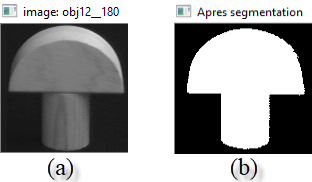
\includegraphics[width=0.5\textwidth]{Figures/segmentation.png} 
	\caption{Segmentation par seuillage de notre système.}
\end{figure}
%-----------------------------------
%	SECTION 5
%-----------------------------------
\section{Systèmes de recherche d'image par contenu (CBIR)}
Les chercheurs dans le domaine de la vision par ordinateur se posent le problème de l'indexation automatique des images par leur contenu, qui permet la recherche d'images par le
contenu (CBIR).\\

CBIR (Content Based Image Retrieval) est un système qui utilise des contenus{\tiny } visuels pour récupérer des images à partir d'une base de données d'images. Ce système est devenu indispensable parce qu'il peut effectivement surmonter les problèmes d'un TBIR (Text Based Image Retrieval). Dans le CBIR, le contenu visuel est extrait par plusieurs techniques:
histogramme, segmentation... Il est également décrit par le vecteur de caractéristiques multidimensionnel. En effet, Le CBIR diffère de la recherche d’information textuelle essentiellement par le fait que les bases de données d’images sont non-structurées, les images numériques n'étant que des matrices d'intensités de pixels, sans signification inhérente les unes par rapport aux autres. Donc avant même de commencer à faire des hypothèses sur le contenu de l'image, une des questions clé dans tout type de traitement d’image est l’extraction de l’information utile à partir de ces matrices de pixels car la performance du système de recherche d'images basées sur le contenu est principalement influencée par la qualité et la pertinence du vecteur de caractéristiques. \\

\subsection{Principe de la recherche d’images par contenu}
Les premiers moteurs de recherche d’images sont basés sur des textes et des mots-clés attribués à chaque image pour l'identifier, mais cette méthode a comme inconvénient que le résultat de recherche contient beaucoup des images qui ne sont pas nécessaires. Pour cela, les spécialistes ont travaillé sur une autre méthode, des systèmes adaptés pour l'approche « basé sur le contenu » (content-based, en Anglais) qui se propose de représenter les images en fonction de leur contenu.\\

Le principe général de la recherche d'image par le contenu comporte deux étapes:
\begin{itemize}
	\item  \textbf{Etape d'indexation (offline):} L'indexation est un ensemble de processus aboutissant à la
	construction d’un vecteur numérique appelé descripteur visuel de l’image.
	Dans cette étape hors ligne, le système commence	par le pré-traitement de l'image, c’est-à-dire l'extraction automatique des	attributs physique à partir des images de la base pour qu'ils doivent être compréhensible par la machine, cette opération peut être nommée "calcul de signature". Après la gestion et l'organisation de ces informations, le système stocke les signatures calculées dans une nouvelle base d'images appelée "base d'index" ou "base de signatures".
	
	\item \textbf{Etape de recherche (online):} La seconde phase, dite de recherche se déroule en ligne. L'utilisateur soumet une image comme requête. Le système calcule le vecteur descripteur (signature)  selon le même mode que lors de la première phase d'indexation. Ainsi, cette signature est comparé à l'ensemble des signatures préalablement stockés dans la base d'index pour en ramener les images les plus semblables à la requête ordonnées en fonction de la similarité à l’aide d’une mesure de distance..
\end{itemize}

\begin{figure}[H]
	    \label{fig:cbir_principe}
		\centering
		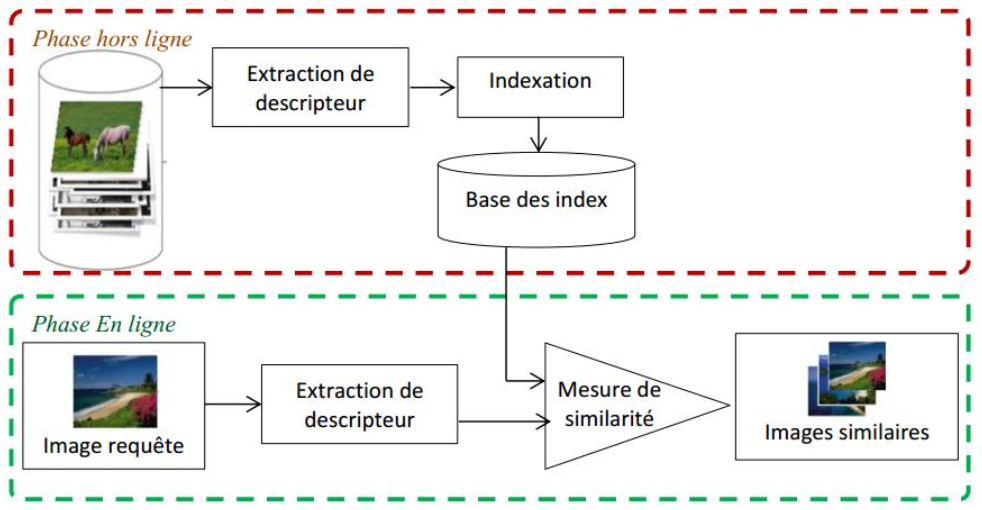
\includegraphics[width=0.7\textwidth]{Figures/cbir_principe} % Include the image .png
		\caption{ Architecture d'un système d'indexation et de recherche d'images.}
\end{figure}

Lors de la phase d'indexation, le calcul de descripteur consiste en l'extraction de caractéristiques visuelles des images telles que:
\begin{itemize}
	\item la texture (filtre de Gabor, transformée en ondelettes discrète…)
	\item la couleur (la segmentation, les points d’intérêts, les régions d’intérêts,
	histogramme de couleurs, histogrammes dans l'espace RGB ou dans TSV, …),
	\item les formes (descripteurs de Fourier, Les moments de Zernike, …),
	\item une combinaison de plusieurs de ces caractéristiques.
\end{itemize}

Ces caractéristiques sont dites de bas-niveau, car elles sont très proches du contenu signal (pixel), et ne véhiculent pas de sémantique particulière sur l'image.\\


\subsection{La base d’images}
La gestion de bases de données désigne la branche de l’informatique qui étudie le stockage et l’interrogation des données numériques. Une base de données informatique est donc un ensemble d’informations numériques stockées selon un modèle dans le but de les conserver, de les enrichir et de les interroger avec la garantie de l’intégrité de ces données [Jerome05]. Généralement, les systèmes de recherche d’images incluent deux bases différentes, la première collecte les images brutes, c’est-à-dire les images non traitées, et la deuxième gère les signatures des images indexées.\\

Ils existent plusieurs bases d’images sur Internet dont la plupart sont librement utilisées. Différentes par leur contenu, chaque base possède des images groupées en plusieurs classes bien définies où chaque image  n’appartient qu’à une seule classe. Généralement, les développeurs utilisent ces bases pour tester les algorithmes de recherche d’images mis en œuvre afin d’évaluer et valider leurs systèmes.\\

Cette section présente les bases d’images les plus utilisées dans le domaine de recherche d’image par le contenu :


\textbf{Columbia Object Image Library (COIL-100):}
C’est une Bibliothèque d’images de l’université de Columbia, elle a été créée en 1996. Cette base d’images est très connue pour la reconnaissance des objets. Il y a deux bases d’images COIL : COIL-20 qui contient des images en niveaux de gris prises à partir de 20 objets différents et COIL-100 qui contient des images en couleurs prises à partir de 100 objets différents. Les deux bases d’images consistent en des images prises à partir des objets 3D avec des positions différentes. La base COIL-100 a 7200 images en couleurs (100 objets x72 images/objet). Chaque image a une taille de 128x128 pixels. La base de Wang est disponible à l’adresse : \href{https://www1.cs.columbia.edu/CAVE/software/softlib/coil-100.php}{COIL-100}.

\begin{figure}[H]
	\centering
	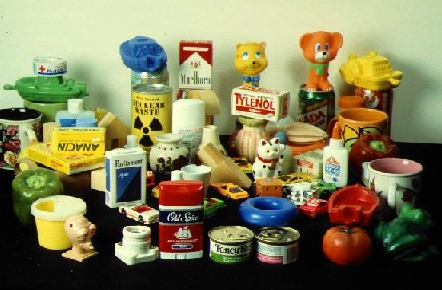
\includegraphics[width=0.5\textwidth]{coil} 
	\caption{Objets utilisés dans COIL-100.}
\end{figure}

\textbf{Corel-1000 - Wang:}
La base d’images de Wang est un sous-ensemble de la base d’images
Corel. Elle a été créée par le groupe du professeur Wang de l'université d'état de Pennsylvanie dans le but de faire des expériences de classification.
Cette base d’images contient 1000 images en couleurs. Ces images ont été divisées en 10 classes de 100 images. Les thèmes représentés par les 10 classes sont : monuments, plage, autobus, dinosaures, aliments, éléphants, fleurs, chevaux, montagnes et l’Afrique.
La base de Wang est disponible à l’adresse : \href{http://wang.ist.psu.edu/}{WANG}.
\begin{figure}[H]
	\centering
	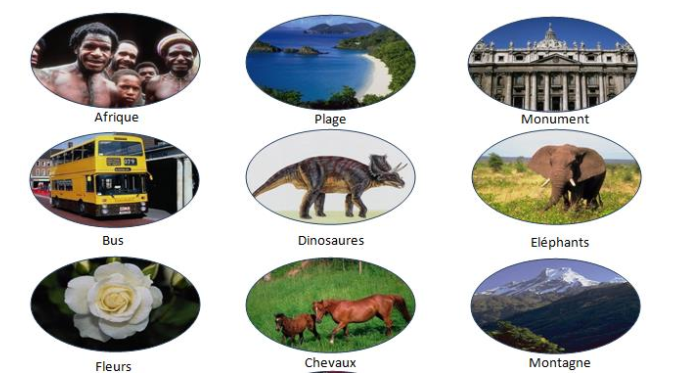
\includegraphics[width=0.6\textwidth]{wang} 
	\caption{Quelques images de la base d’image WANG.}
\end{figure}

\textbf{La base INRIA:}
Est un ensemble d’images photos personnelles de vacances. Cette base contient aussi des versions d’images changées à travers la rotation, le point de vue et d’illumination, flou, ...etc.

L’ensemble de données contient 500 groupes d’images, qui représentent une scène ou un objet distinct. La première image de chaque groupe est l’image de requête et les résultats corrects de récupération sont les autres images du groupe. La taille totale du corpus est : 1491 images au total : 500 questions et le reste ce sont les images de l’index. 

\begin{figure}[H]
	\centering
	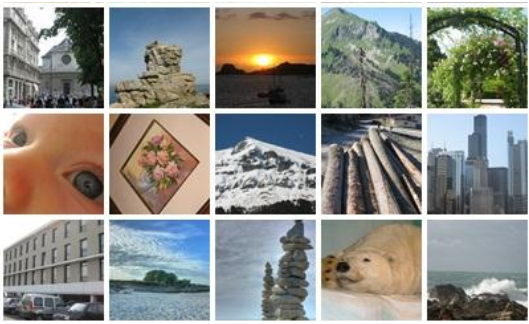
\includegraphics[width=0.6\textwidth]{inria} 
	\caption{Quelques images de la base d’image INRIA.}
\end{figure}


\subsection{Les requêtes}
La plupart des systèmes de recherche d’images disposent d'une interface graphique permettant aux utilisateurs d'effectuer une recherche par le biais d'une requête. L’utilisateur peut spécifier directement les attributs de bas niveau de l'image cible dans sa requête, interroger le système en esquissant un croquis, ou bien en présentant au système une image exemple de ce qu'il recherche.

Voici les quatre façons (types) pour faire une requête dans un système de recherche d'images :

\begin{enumerate}
	\item \textbf{Requête par description :}
	Dans cette méthode, l’utilisateur indique ce qu’il veut en termes de descripteur visuel, il décrit l’image qu’il souhaite obtenir en fonction de ces caractéristiques visuelles comme la couleur et la texture (par exemple, chercher une image contenant $40\%$ de bleu en haut, $20\%$ de vert en bas).
	Ces caractéristiques sont classées dans un répertoire dépend de moteur de
	recherche.
	
	\item \textbf{Requête par mots clés :}
	L’utilisateur exprime ses besoins en fournissant un ou plusieurs mots clés, qui peuvent être combinés à l'aide de connecteurs logiques tels que et, ou et non. Dans cette méthode, les systèmes se basent, en plus d'indexation par contenu, sur l’indexation textuelle manuelle d'image pour filtrer le résultat. Plusieurs moteurs de recherche d’images en ligne utilisent cette approche telle que Google et Yahoo, mais elle reste une façon de recherche fatigante surtout avec des bases d'images volumineuses [ZZ18].
	\begin{figure}[H]
		\centering
		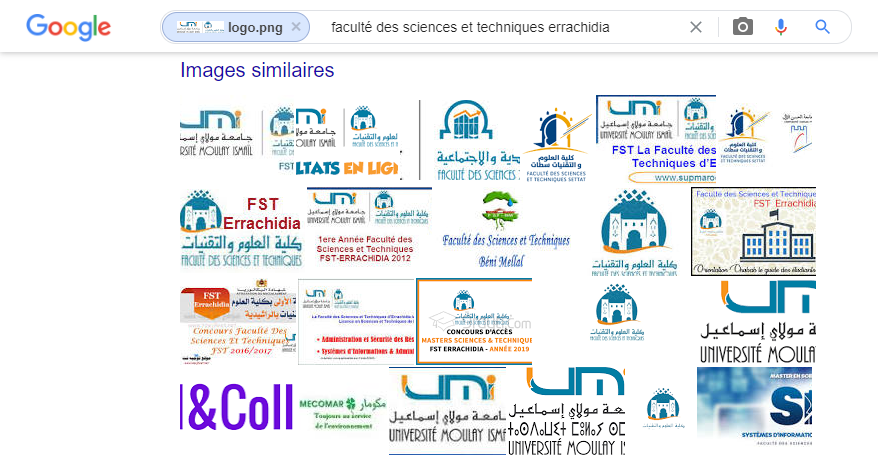
\includegraphics[width=0.6\textwidth]{fstelook} 
		\caption{Capture d’écran d’une recherche effectuée sur Google avec des mot-clés et une image, réalisée le 27/06/2020.}
	\end{figure}

	\item \textbf{Requête par esquisse :} Puisque les deux méthodes précédentes ont des désavantages, les chercheurs développent d'autres approches pour renforcer les moteurs
	de recherche d’images tel que la requête par esquisse ou bien par crayonnage. Dans cette approche, le système propose à l’utilisateur un ensemble d'outils de dessin et une palette de couleurs qui lui permet de spécifier sa requête en forme d’un sketch. Après, le système calcule les ressemblances entre le dessin et les images de sa base.
		\begin{figure}[H]
			\centering
			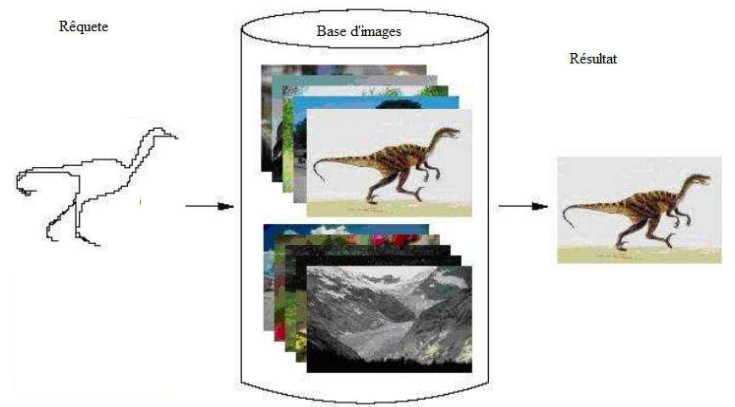
\includegraphics[width=0.6\textwidth]{croquis} 
			\caption{Exemple de requête par esquisse.}
		\end{figure}
	
	\item \textbf{Requête par image exemple :}
	Dans ce type de requête, il y a deux façons de commencer la
	recherche. La première consiste que l’utilisateur dispose d’une image de référence de ce qu’il cherche et la fournit au système comme un exemple.
	Dans la deuxième façon, le système montre à l’utilisateur quelques classes d’images, l’utilisateur sélectionne une classe et parcourt la liste d’images affichées par le système, puis il choisit une image de la liste comme étant une requête.
	Donc le système a besoin de comparer un exemple de même type (image) avec la base pour produire les items similaires. Cette méthode est simple, naturelle et ne nécessite pas de connaissances approfondies pour manipuler le système. Elle est donc bien adaptée à un utilisateur non spécialiste. C'est le type intégrer par notre système.
	
\end{enumerate}

\subsection{Mesures d’évaluation d’un système CBIR}
Une évaluation qui permet de mesurer la qualité d’un système de
recherche d’images est une étape nécessaire avant l’exécution de ce système. D’une façon générale, la recherche d’images par le contenu est une branche de la recherche d’informations, les objectives et les mesures d’évaluation du système qui ont été faits pour la recherche d’informations sont les mêmes
pour la recherche d’images. Par ailleurs, pour mesurer la performance d’un système, il faut qu'on dispose d'un ensemble d’images de test et d'une vérité terraine  (ground truth),
c'est-à-dire que nous savons préalablement quelles sont les images
appropriées à l'image requête dans la base d'images. Pour une évaluation significative il est important d'avoir un ensemble représentatif d'images requêtes. Ceci veut dire que l'ensemble des images requêtes doit être choisi d’une manière minutieuse [Khouloud09].
Dans l’exploitation de ces systèmes, les utilisateurs s’intéressent à deux objectifs principaux, un temps de réponse court et des résultats pertinents  du système, c'est-à-dire qu’il peut retrouver tous les images pertinentes et éliminer les images non pertinentes.


Dans cette section nous allons d’écrire les mesures les plus utilisées.

\subsubsection{Rappel et précision (en anglais : Recall and Precision)}

Dans les systèmes de recherche d’informations, afin de définir si une
information est pertinente ou non, on a besoin d’experts dans le domaine.
Dans les systèmes de recherche d’images, une image est pertinente pour une
requête si les deux images sont dans la même classe. C’est pourquoi dans
l’étape de préparation de la base d’images pour évaluer, on doit faire des
annotations. L’annotation est un processus qui permet aux utilisateurs de
choisir des mots clés correspondants à chaque image. Après l’annotation, on va classifier les images en classes appropriées. Si des images ne contiennent pas beaucoup d’objets, c’est facile de les classifier dans ces classes. Mais si les images contiennent beaucoup d’objets, la tâche de classification devient de plus en plus difficile. Dans ce cas-là, chaque image appartient à plusieurs classes .

\begin{itemize}
	\item \textbf{Le rappel :}
	Le rappel représente le rapport entre le nombre d’images pertinentes à la requête dans l’ensemble des images trouvées par le système et le nombre d’images pertinentes dans la base d’images.
	\begin{equation}
		R = \frac{| A \cap B|}{| A |} = \frac{\text{Nombre d'images pértinentes retrouvées}}{\text{Nombre total d'images pértinentes}}
	\end{equation}
	Où A l’ensemble des images résultat pertinentes pour une requête donnée et B l’ensemble des images résultat retournées par le système.
	
	\item \textbf{La précision :}
	La précision représente le rapport entre le nombre d’images pertinentes à la requête dans l’ensemble des images trouvées et le nombre d’images trouvées.
	
	\begin{equation}
	P = \frac{| A \cap B|}{| B |} = \frac{\text{Nombre d'images pértinentes retrouvées}}{\text{Nombre total d'images retrouvées}}
	\end{equation}
\end{itemize}

\begin{figure}[H]
	\centering
	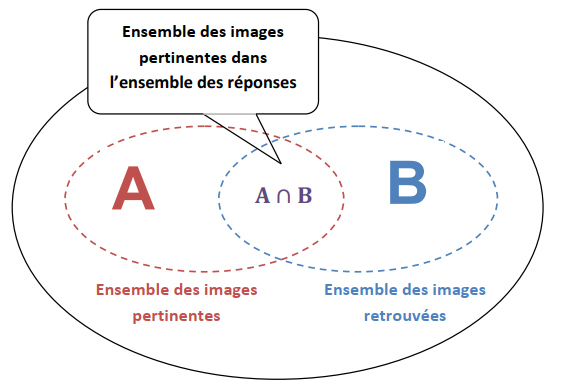
\includegraphics[width=0.4\textwidth]{recall} 
	\caption{ Le rappel et la précision pour une requête.}
\end{figure}

La précision et le rappel sont compris entre 0 et 1. Par exemple, si on utilise la base d’images de Wang qui contient 100 images par la classe " fleurs ", et le moteur de recherche retourne 8 images appropriées parmi 10 images trouvées, le rappel et la précision seront :
Le rappel = 8/100 = 0.08 ; la précision = 8/10 = 0.8.
Les deux métriques "rappel et précision" s’utilisent conjointement pour
l’évaluation des performances des systèmes de recherche. Les valeurs de ces deux métriques reflètent le point de vue de l’utilisateur (si le rappel est faible, une partie de l’information pertinente ne lui sera pas accessible, et si la précision est faible, l’utilisateur ne sera pas satisfait à cause de la forte concentration des informations non-pertinentes fournies dans les résultats).
Dans les deux cas, le système ne répond pas aux attentes des utilisateurs à retourner l’information utile et pertinente, et par la suite, il est nonperformant. Le cas idéal est d’avoir la valeur de précision et rappel
respectivement égale à un [Imane12].

\subsubsection{La courbe rappel/précision}
En pratique, le calcul d’une paire de valeurs (rappel et précision) ne
peut pas indiquer la performance du système. Donc il est nécessaire
d’utiliser plusieurs requêtes afin de donner une distribution de
rappel/précision sous forme d’une courbe, où chaque point de cette courbe
représente la précision moyenne calculée pour toutes les images
correspondant à ce niveau de rappel. Ce calcul statistique permet de suivre
la qualité du résultat en fonction du nombre d’images affichées par le
système en réponse à une requête.
La figure 1.22 donne un exemple de courbe de rappel et précision.
\begin{figure}[H]
	\centering
	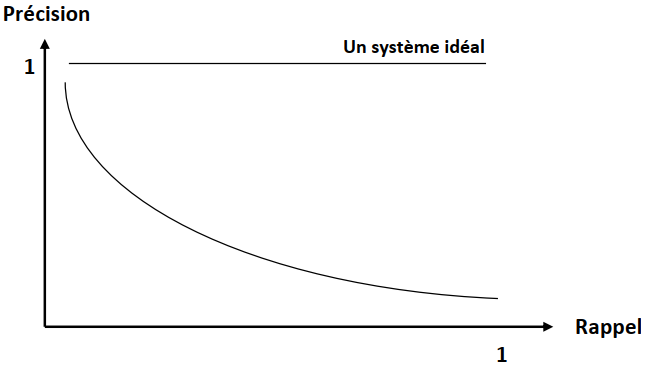
\includegraphics[width=0.4\textwidth]{courve} 
	\caption{Une courbe de rappel/précision.}
\end{figure}

Le rappel et la précision sont très utiles parce qu’ils nous permettent
d’évaluer quantitativement la qualité de la réponse globale. Mais ils ont ces quatre désavantages.
\begin{itemize}
	\item L’estimation de la valeur maximum de rappel exige de savoir toutes les connaissances de la base d’images. Quand la base d’images devient de plus en plus grande, ces connaissances ne sont pas disponibles, ce qui veut dire que l’évaluation n’est pas bien estimée.
	\item Le rappel et la précision sont reliés. Donc dans quelques cas, les deux mesures ne sont pas suffisantes. L’utilisation d’autres mesures qui combinent le rappel et précision pourrait être plus appropriée.
	%\item Ces mesures travaillent bien sur un ensemble de requêtes par lots. Cependant, les systèmes modernes ne travaillent pas dans ce mode.
	%\item Le rappel et la précision sont faciles à définir quand l’ordre des images est linéaire. Ces mesures ne sont pas appropriées pour les systèmes qui ont un ordre faible.
\end{itemize}

A cause de ces désavantages, d’autres mesures qui sont plus appropriées
doivent être utilisées comme :

\begin{itemize}
	\item \textbf{La moyenne harmonique ou F-mesure:} Mathématiquement, la moyenne 
	harmonique H est utilisée lorsqu'on
	veut déterminer un rapport moyen,
	dans un domaine où il existe des 
	liens de proportionnalité inverses.
	Dans notre cas, la moyenne harmonique
	combine le rappel et la précision en un
	nombre\\ réel compris entre 0 et 1 
	\begin{equation}
	    F = \frac{2}{\frac{1}{R}+\frac{1}{P}} = \frac{2\times R \times P}{R+P}
	\end{equation}
	Où :\\
	R : la valeur du rappel.  \space\space	P : la valeur de la précision.
	
	
	Si cette valeur vaut 0 ça veut dire
	qu’aucune image pertinente n’a été
	retrouvée. Si la valeur vaut 1, toutes
	les images pertinentes ont été
	retrouvées. De plus, cette mesure a 
	une valeur élevée quand le rappel et la
	précision sont élevés.
	
	\item\textbf{ La mesure E :}

	\begin{equation}
			 E = \frac{1+b^2}{\frac{b^2}{R}+\frac{1}{P}}
	\end{equation}
	
	Elle permet à l’utilisateur d’indiquer 
	s’il est intéressé par le rappel ou la précision.
	Si l’utilisateur choisit b > 1, ça veut dire qu’il s’intéresse plus à la précision.
	Et s’il choisit b < 1, ça veut dire qu’il donne la priorité au rappel plus qu’à la précision.    
\end{itemize}
		
		
%
%
%
%Une fois ces caractéristiques extraites, la comparaison consiste généralement à définir diverses distances entre ces caractéristiques, et de définir une mesure de similarité globale
%entre deux images. Au moyen de cette mesure de similarité et d'une image requête, on peut alors calculer l'ensemble des mesures de similarités entre cette image requête et l'ensemble des images de la base d'images. On peut alors ordonner les images de la base suivant leur score, et présenter le résultat à l'utilisateur, les images de plus grand score étant considérées comme les plus similaires.\\
%
%Ce genre de système ne nécessite pas forcément une image requête pour rechercher d'autres images. Par exemple, il est possible de rechercher des images plutôt bleues, ou alors de dessiner une forme et demander de chercher toutes les images qui possèdent un objet de forme similaire.
%
%
%
%Une des étapes essentielles en analyse d'images par le contenu est l'extraction d'une description de bas niveau de l’image. Cette description est une représentation numérique (analyse statistique, analyse quantitative, ...) des caractéristiques visuelles de l'image, généralement sous la forme d’un vecteur ou d’un ensemble de vecteurs.
%Cette description doit avoir deux caractéristiques importantes :
%\begin{itemize}
%	\item elle doit conserver suffisamment d’information pour être discriminante, c’est-à-dire différencier deux images avec un contenu visuel différent;
%	\item elle doit être la plus invariante possible (aux bruits; aux variations d’échelle; aux variations de contraste; aux déformations; etc) pour pouvoir généraliser le contenu visuel d’une image à une autre image qui n’est pas identique.
%\end{itemize}
%
%
%Nous présentons dans la suite les différentes familles de descripteurs.
%
%
%\subsection{Descripteur globaux et descripteurs locaux}
%On peut résumer l’ensemble des informations visuelles de l’image en un unique descripteur
%global, ou plusieurs descripteurs locaux caractérisant chacun une partie de l’image. Les
%techniques modernes en imagerie tendent à privilégier les descripteurs locaux aux globaux car
%les descripteurs locaux sont plus efficaces et ils permettent une recherche plus fine et
%absorbent mieux certaines variations.
%
%\subsubsection{Descripteurs globaux}
%Dans le cas de descripteurs globaux, un seule descripteur décrit la totalité de l’image, cela
%les rend robustes au bruit qui peut affecter le signal, les histogrammes de couleur et des
%niveaux de gris en sont des exemples classiques [Stricker 94]. De nombreux descripteurs
%globaux sont également basés sur la texture et la couleur. La couleur aussi fait partie des
%premières primitives visuelles utilisées. Le plus simple des descripteurs globaux basés sur la
%couleur consiste à construire l’histogramme des couleurs.
%L’inconvénient de ces descripteurs est qu’ils ne permettent pas de distinguer des parties de
%l’image, ils ne distinguent pas, par exemple, les objets dans l’image, sauf dans le cas où
%l’image ne contient qu’un seule objet sur un fond uni.
%
%\subsubsection{Descripteurs locaux}
%Les descripteurs locaux s’associent à une partie/région de l’image qu’on commence par
%détecter avant de calculer le descripteur, cette partie peut concerner un objet par exemple, la
%détection se fait indépendamment de la position dans l’image, ce qui assure l’invariance par
%translation, rotation, etc .
%
%Les descripteurs locaux sont de nos jours les caractéristiques visuelles les plus couramment
%utilisées en analyse d’image par le contenu. Ils permettent de décrire l’ensemble des
%informations visuelles d’une région de l’image en un descripteur (vecteur). La région
%d’extraction est appelée région d’intérêt et elle est généralement centrée sur un point d’intérêt
%Les descripteurs locaux ont une très bonne capacité de discrimination pour déterminer si
%deux régions sont similaires ou dissimilaires. Cela les rends particulièrement utiles en vision
%par ordinateur, notamment pour de la mise en correspondance de points d’intérêts. Ils sont
%utilisés en : odométrie visuelle [Nistér 04] ; reconstruction 3D [Mouragnon 06] ; détection
%d’objets [Lowe 99] ; recherche d’images par le contenu [Perronnin 10], [Negrel 14] ; etc.
%Dans le chapitre suivant, nous présentons un descripteur local basé sur la segmentation par
%k-means.
%
%\subsection{Combinaison des descripteurs}
%
%Les attributs: couleur, texture, forme décrivent les images par leur contenu visuel. La
%combinaison de ces attributs peut être mieux caractérisée le contenu. Il est donc intéressant de
%combiner ces différents attributs pour une recherche plus efficace et plus discriminante. Les
%problèmes qui se posent lors de la combinaison de ces différents attributs pour la recherche et
%l’indexation sont au moins de trois ordres :
%\begin{itemize}
%	\item L'espace de description : Le choix de l'espace de description consiste à rechercher les
%	attributs visuels significatifs de la base de données d'images, l'ensemble de ces
%	attributs étant représenté par un nuage de points dans un espace dimensionnel haut,
%	alors les vecteurs contiennent plusieurs attributs, un problème qui se pose est celui de
%	la dimension de l'espace de description. Ce problème est connu dans la communauté
%	des bases de données par la malédiction de la dimension, lorsque le nombre de
%	dimensions augmente, le volume de l'espace croît rapidement si bien que les données
%	se retrouvent « isolées » et deviennent éparses.
%	\item La mesure de la similarité : Il s'agit d'une étape essentielle dans tout système de
%	recherche. Dans le cas où les images sont décrites par différents attributs, une solution
%	classique pour mesurer la similarité est de calculer séparément les mesures de
%	similarité pour chaque attribut et de déduire ensuite une mesure composite de la
%	similarité globale entre les images. Cela suppose évidemment que les différents
%	attributs sont indexés séparément (avec des structures d'index séparées). Dans la base de données, il y a peu de méthodes qui utilisent plusieurs index pour structurer les
%	données. Une autre difficulté liée à la similitude est de déterminer comment combiner
%	plusieurs mesures souvent définies sur des domaines différents, avec des dynamiques
%	différentes, des degrés d'importance différents, surtout pour l'utilisateur, mais aussi de
%	natures différentes.
%	\item Structuration : la phase de construction d'une structure d'index est une étape utile dans
%	le cas où les données sont volumineuses et appartiennent à un grand espace de
%	description. Il s'agit de structurer les nuages de points relatifs aux descripteurs des
%	images et de les stocker efficacement dans une machine. Cette tâche de structuration
%	peut s'avérer difficile dans le cas où les données à structurer sont de nature hétérogène.
%	La difficulté réside dans le choix de la distance à utiliser pour structurer (mise en place
%	d'un index) et dans la standardisation des différents types de données.
%\end{itemize}
%
%

%----------------------------------------------------------------------------------------
%	SECTION 2
%----------------------------------------------------------------------------------------


\section{Conclusion}
Ce chapitre a fait l’état de l’art sans exhaustivité des différentes notions de base qui décrivent le domaine de traitement de l'image numérique et les systèmes de  recherche d'images par le contenu ainsi que les approches correspondantes. Nous avons abordé premièrement une brève définition sur l’image numérique et ces caractéristiques. Ensuite, nous avons étudié le principe de traitement d’image avec ces étapes tel que le filtrage et la segmentation. Aussi, nous avons défini brièvement le principe d’un système de recherche d’images par le contenu (CBIR) ainsi que l’architecture de fonctionnement. Ensuite, nous avons présenté les différentes bases d’images les plus utilisées, les types de requête et la représentation des images dans ces systèmes. A la fin de ce chapitre, nous avons aussi montré les mesures utilisées pour évaluer un CBIR comme le rappel et la précision.\\

Le chapitre suivant sera consacré à deux étapes fondamentales dans la
recherche d’images par le contenu. L’extraction d’attributs pour la création des vecteurs descripteurs (signatures) et la mesure de similarité entre une image requête et les images de la base d'index.

